\documentclass{ceadar_article}
\usepackage{graphicx} % This lets you include figures
\usepackage{mdframed}
\usepackage{tabularx} % This lets you draw tables
\usepackage{float} % This prevents LaTeX from re-positioning the tables.
\usepackage{dirtytalk} % This lets you quote
\usepackage{longtable, tabu}

\restylefloat{table}

\definecolor{mygrey}{gray}{0.8}


\surroundwithmdframed[linewidth=0pt,backgroundcolor=mygrey]{verbatim}

\graphicspath{{reference/}}

\begin{document}


\title{Blockchain Scalability Testing (WP-3) Report}

\abstract{
Blockchain Scalability Testing - report (WP-3).
}

% Data for the front page table
\doctype{Scalability report}
\projecttitle{Blockchain Scalability Testing (WP-3) - Report}
\workpackage{3}
\author{Prabhakaran AK, Saad Shahid, Ois\'{i}n Boydell}
\docstate{Draft}
\deliverydate{July 2020}
\docversion{0.1}

\maketitle

\newpage


\section{Introduction}

Blockchain scalability testing predicts the performance of the blockchain network while the consortium grows over the period of time. As the number of nodes in the consortium grows, volume of the transactions going through the network is expected to grow as well. 

This document presents the result of the scalability testing. Several tests are run with varying volume and frequency of the transaction and the results are compared and presented for the better understanding of users.
\newline

\section{Tool}
For the scalability testing purpose we are going to user Hyperledger caliper\footnote{\url{https://www.hyperledger.org/projects/caliper}}. It supports various version of hyperledger fabric. For this document purpose, Hyperledger caliper V0.3 will be used.

\subsection{Requirements}
The requirement is to analyze the scalability performance of a smart contract in a blockchain network. The scalability check will determine the latency variation against the variation in transaction volume and throughput.


\subsection{Assumptions}
The following are the assumptions for this test run
\begin{itemize}
    \item This document use Hyperledger caliper verion 0.3.
    \item Full size of network is assumed to be 136 Organizations
    \begin{itemize}
        \item Distributor - 1
        \item Publishers - 111
        \item Providers - 24
    \end{itemize}
    \item It covers the product key and product key batch request smart contract
    \item Since both the smart contract have similar overload, for testing purpose we will use 
    \begin{itemize}
        \item Product key smart contract
        \item Create, Allocate and Query method
    \end{itemize}
    \item We will run the experiments against the following metrics
    \newline Transaction volume - Fixed at 10,000

       \begin{tabular}{|l|l|l|l|l|l|}
\hline
\# of nodes / TPS                   & 10  & 25  & 50   & 100 & 500 \\ \hline
07(5\%)                             &     &     &      &     &      \\ \hline
27 (20\%)                           &     &     &      &     &      \\ \hline
68 (50\%)                           &     &     &      &     &      \\ \hline
102 (75\%)                          &     &     &      &     &      \\ \hline
136 (100\%)                         &     &     &      &     &      \\ \hline
\end{tabular}
    \item The results of the experiments will be consolidated into excel sheet and presented in a chart format
\end{itemize}


\subsection{About Hyperledger Caliper}
We are going to use Hyperledger Caliper \cite{hyperledgerCaliper}, a blockchain bench-mark tool to measure the performance of the blockchain implementation with a set of predefined use cases. \newline
Hyperledger caliper is a blockchain performance bench-marking tool from the Linux foundation. 

\subsection{Why Hyperledger Caliper}
Caliper has a defined Performance \& Scalability Working Group (PSWG) \cite{pswg} which contains definitions and metrics for the blockchain network bench-marking. \newline
It has support for multiple versions of hyperledger fabric which is our blockchain platform for the present use case\newline
Caliper helps us to determine the various-metrics for given volume of transactions at defined throughput.

\subsection {Performance \& Scalability Working Group - metrics}
The metrics that are defined by the PSWG of Hyperledger caliper are as follows:

\subsubsection{Success Rate} 
Measures all successful and failed transactions for a test cycle.
\begin{itemize}
    \item This metrics is based on the volume of the transactions.
    \item Caliper allows users to configure the transaction volume for the testing.
    \item Caliper final report includes the success and failure rate for the given volume of transactions.
\end{itemize}


\subsubsection{Transaction \& Read Latency} 
Measures the time for an issued transaction to be completed and a response being available to the application that issued the transaction. 

\begin{itemize}
    \item This metrics is based on the time taken for one single transaction in seconds.
    \item Latency is the output by hyperledger caliper for given volume of transactions at defined throughput.
    \item Maximum, minimum and average latency in seconds for the test cycle is provided.
\end{itemize}

\subsubsection{Transaction \& Read Throughput} 
Measures the flow rate of all transactions through the system, in transactions per second, during the a cycle. 
\begin{itemize}
    \item This metrics defines the flow rate of transaction into the blockchain system.
    \item Throughput can be configured at caliper.
    \item Unit of measurement for throughput is Transactions per second (TPS).
    \item Various types of throughput feeding is possible in caliper.
    \begin{itemize}
       \item fixed-rate : Fixed rate of throughput is maintained from start to end of the transaction volume.
       \item linear-rate : Variable rate between beginning and towards end of the transaction volume.
       \item composite-rate: Composite rate allows both fixed rate and linear rate throughput to be used on given transaction volume.
     \end{itemize}
   
\end{itemize}

\subsubsection{Dependency Latency vs Throughput}
Hyperledger caliper provides sample smart contracts to run the scalability check, and based on the results of running it against different transaction volume and throughput we arrived at the following assumption:

\begin{itemize}
    \item Latency increases linearly with number of nodes in the network.
    \item Throughput is configurable for each test run.
    \item Latency increases when the volume of the transaction and throughput is increased. 
\end{itemize}

The same will be verified against each of our smart contract across WP-6 in phases.

\subsection{Resource Consumption} Measures the following resource parameters of the blockchain network
\begin{itemize}
    \item Max. and Min, memory - Memory used in MegaBytes
    \item CPU resource consumption - CPU usage in percentage
    \item I/O traffic - KiloBytes/ MegaBytes
\end{itemize}

\section{Network setup}
The blockchain network structure on which the experiments will be run are as follows
\subsection{Version}
Hyperledger Fabric version 1.4.4 will be used
\subsection {Consensus}
RAFT consensus mechanism with two orderer node will be used
\subsection {Organizations}
A total of 136 organizations will be used with a single peer structure. All the organizations will be hosted in Azure cloud 

\section{Experiment}
The scalablity experiment will be executed as follows

\subsection {Transaction volume}
A total of 10000 transactions will be used for each round of experiment. The transaction volume is fixed for all the experiments

\subsection {Throughput}
Totally five sets of throughput will be used in a fixed rate manner. 
\begin{itemize}
    \item 10 TPS
    \item 25 TPS
    \item 50 TPS
    \item 100 TPS
    \item 500 TPS
\end{itemize}

\subsection {Node count}
Totally 136 nodes will be used under that assumption, the network can contain a maximum of one distributor, 111 publishers and 24 providers. The node count will be spread across for experiment as follows

\begin{itemize}
    \item  1 distributor - 3 publishers - 3 providers (5\% of the total size)
    \item  1 distributor - 20 publishers - 7 providers (20\% of the total size)
    \item  1 distributor - 77 publishers - 24 providers (50\% of the total size)
    \item  1 distributor - 20 publishers - 24 providers (75\% of the total size)
    \item  1 distributor - 111 publishers - 24 providers (Full network)
\end{itemize}

\subsection{Plotting the results}

The results from the above experiments are plotted in five different charts. A chart for each scale set of nodes mentioned in section 4.3 will be plotted. The chart will contain the throughput in TPS plotted vs latency in seconds.
\newline
Each round of experiment will give two sets of latency values, min latency and max latency. For each throughput mentioned in section 4.2, min latency, max latency and average latency will be marked. 

\subsubsection{Results for 5\% of the network scale}
    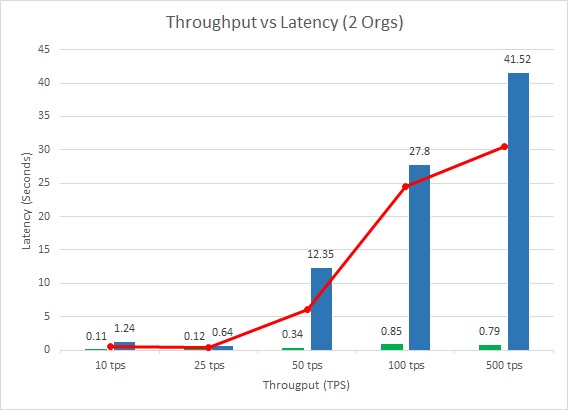
\includegraphics[width=17cm,height=11cm]{ChartSample}
    
\subsubsection{Graph for 20\% of the network scale}
    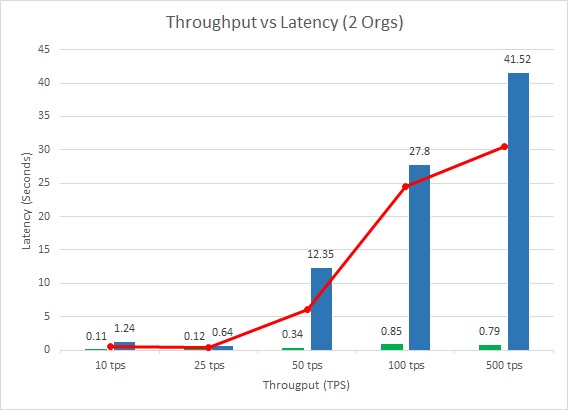
\includegraphics[width=17cm,height=11cm]{ChartSample}

\subsubsection{Graph for 50\% of the network scale}
    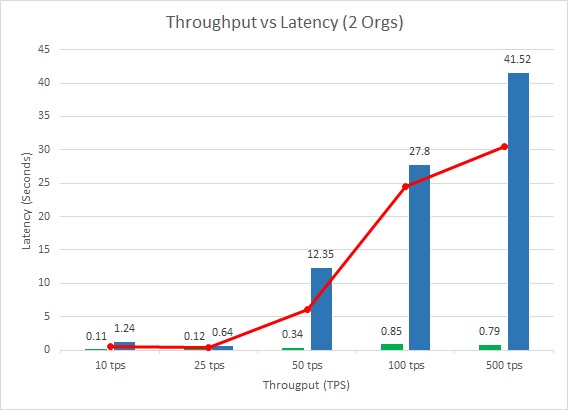
\includegraphics[width=17cm,height=11cm]{ChartSample}
  
\subsubsection{Graph for 75\% of the network scale}
    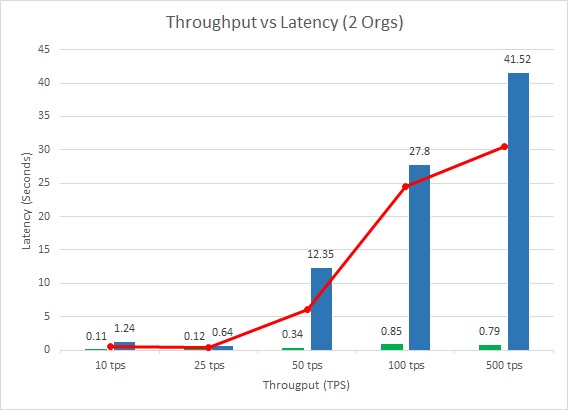
\includegraphics[width=17cm,height=11cm]{ChartSample}

\subsubsection{Graph for full network scale}
    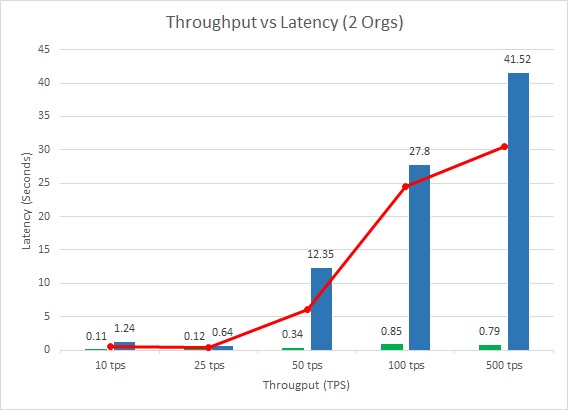
\includegraphics[width=17cm,height=11cm]{ChartSample}


\appendix
\section{Caliper reference}
The caliper reference files used for the experiments can be found at gitlab location
\newline{\url{https://www.hyperledger.org/projects/caliper}
\section{Fabric reference}
The Hyperledger fabric network reference files used for the experiments can be found at gitlab location 
\newline{\url{https://www.hyperledger.org/projects/caliper}

\bibliographystyle{plain}
\addcontentsline{toc}{section}{Bibliography}
\bibliography{wp-3_scalability_proposal.bib}

\end{document}
